\chapter{Verwendete Technologien}\label{cha:used-technologies}

\section{Over The Air Update}\label{sec:ota}

\subsection*{Problemstellung}\label{sec:problem}
Mikrocontroller befinden sich, wenn sie sich in einem laufendem System befinden meist an ungünstigen Orten, an die man nur mit hohem Aufwand gelangt.
Bis jetzt musste man den Computer physisch mit einem Kabel mit dem Mikrocontroller verbinden um neue Firmware auf den Kontroller zu spielen.
OTA ermöglicht es den Mikrocontroller über das Netzwerk mit neuer Firmware zu versorgen, dabei muss der selektierte Microcomputer lediglich mit einem Wlan-Router verbunden sein und ein physisches Kabel wird überflüssig.

\subsection*{Wie OTA funktioniert}
Am wichtigsten ist es, dass man die Partitionstabelle an das ausgewählte Programm anpasst. 
Die Standard-Partitionstabelle ist je nach Hersteller anders. Um OTA zu ermöglichen ist es notwendig im Partitionstabelle mindestens eine, ausreichend große, OTA-Partition zu vergeben. Dabei ist es wichtig, dass diese Partition ausreichend Speicher für die gewünschte Firmware hat.

Bei dem OTA-Vorgang wird zuerst die Config-Datei, des jeweiligen Mikrocontrollers, ausgelesen. In dierser Config-Datei steht auch welches Firmware sich OTA herunterladen soll. Nun überprüft der Mikrocontroller ob die Firmware-Version des Servers neuer ist als die, die der Controller bereits besitzt, ist dies der Fall wird die neue Version heruntergeladen und der Mikrocontroller wird mit der aktuellen Version neu gestartet.

\subsection*{Implementation}
Die ausgewählte Struktur für die Diplomarbeit kann man im folgenden Bild sehr gut sehen.

\begin{figure}[H]
    \begin{center}
        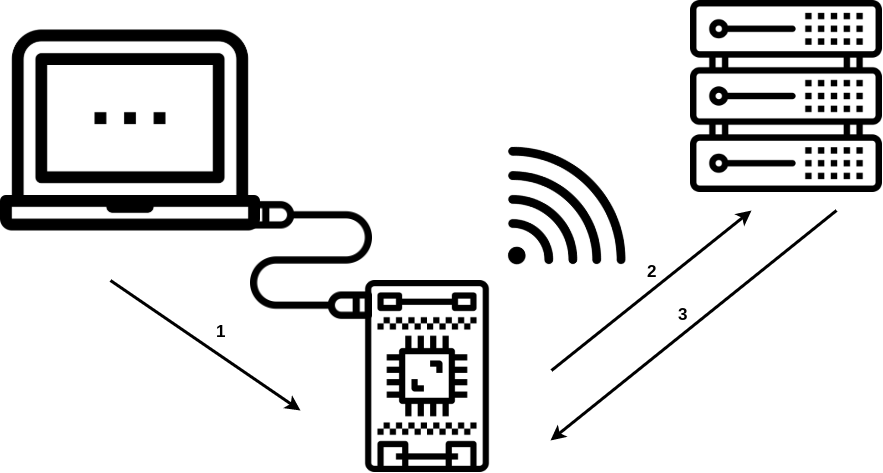
\includegraphics[scale=.5]{images/ota-explanation.png}
        \caption{OTA Erklärung (Quelle: eigene Darstellung)}
    \end{center}    
\end{figure}

\section{Mesh Netzwerk}\label{sec:mesh}

\section{Nodejs}\label{sec:nodejs}

\section{Platform IO}\label{sec:platformio}

\section{Docker}\label{sec:docker}

\section{Docker Compose}\label{sec:docker-compose}

\section{ESP IDF Utility lib}\label{sec:esp-idf-utility-lib}

\section{React}\label{sec:react}

\section{Yarn}\label{sec:yarn}

\section{Webpack}\label{sec:webpack}
